\documentclass{article}
\usepackage{acl}
\usepackage{times}
\usepackage{latexsym}
\usepackage{graphicx}
\usepackage{amsmath}
\usepackage{amssymb}
\usepackage{url}
\usepackage{booktabs}
\usepackage{multirow}
\usepackage{subcaption}
\usepackage{xcolor}
\usepackage{algorithm}
\usepackage{algorithmic}

\title{Mechanistically Disentangling Safety and Innovation: \\ Topological Separation of Conflicting Governance Circuits in LLMs}

\author{
  Seunghyun Yoo \\
  Purdue University \\
  \texttt{yoo236@purdue.edu}
}

\begin{document}
\maketitle

% ============================================================
% ABSTRACT
% ============================================================
\begin{abstract}
Large Language Models (LLMs) aligned for safety often suffer from an ``alignment tax,'' where over-refusal degrades helpfulness \citep{safety_tax2025, rottger2024xstest, orbench2025}. We mechanistically investigate this trade-off within Gemma-2-2B \citep{gemma2_2024} using a contrastive corpus of 1{,}801 AI governance provisions from the AGORA dataset \citep{agora2024}. Our pipeline combines Sparse Autoencoder (SAE) feature decomposition via GemmaScope transcoders \citep{lieberum2024gemma}, rigorous statistical filtering (Global Benjamini-Hochberg FDR correction \citep{benjamini1995controlling} pooling 78{,}575 hypotheses across five layers, with 10{,}000 permutation tests per feature), and causal circuit tracing \citep{ameisen2025circuit}. We isolate 42 statistically significant polarized features at Layer~24---86\% of which survive lexical confound controls---demonstrate their causal necessity via targeted activation steering, and extract cross-layer attribution subgraphs. We confirm our ``Brake and Accelerator'' hypothesis: safety processing invokes topologically deeper ($\mathcal{D}=16$ vs.\ $11$) and \textbf{sparser} checking circuits compared to innovation generation. Our findings provide a mechanistic blueprint that may inform targeted steering strategies aimed at mitigating alignment trade-offs.
\end{abstract}

% ============================================================
% 1. INTRODUCTION
% ============================================================
\section{Introduction}

As AI systems are deployed in high-stakes regulatory environments, developers face a persistent dual mandate: ensure strict safety constraints while fostering innovation and utility. Current alignment methods---RLHF, Constitutional AI, and DPO---often blur these objectives within unified network weights, leading to \textbf{over-refusal}: models conservatively reject benign or creative requests to avoid violating safety bounds \citep{rottger2024xstest, orbench2025}.

The ``safety alignment tax'' has been formally studied: \citet{safety_tax2025} demonstrate that safety alignment systematically diminishes reasoning capabilities, while \citet{nspo2026} propose null-space constrained optimization to mitigate this at the training level. However, these approaches operate without mechanistic understanding of \textit{how} safety and utility are internally represented.

We adopt \textbf{mechanistic interpretability} \citep{elhage2021framework}---the study of internal computational structure. Recent breakthroughs, including the discovery that LLM refusal is mediated by a single direction \citep{arditi2024refusal}, suggest that safety behaviors are localized rather than distributed. We extend this insight by hypothesizing that safety and innovation processing recruit \textit{topologically distinct computational subcircuits}. We propose a \textbf{``Brake and Accelerator''} hypothesis:
\begin{itemize}
    \item \textbf{The Brake (Safety):} Processing safety constraints invokes deeper, highly branched circuits responsible for multi-step condition checking.
    \item \textbf{The Accelerator (Innovation):} Processing innovation incentives uses shallower, linearly structured circuits oriented toward rapid, reward-seeking completions.
\end{itemize}

Our contributions are:
\begin{enumerate}
    \item A domain-grounded contrastive feature discovery pipeline using AGORA \citep{agora2024} policy provisions with rigorous FDR bounding (\S\ref{sec:feature_discovery}).
    \item Causal validation via targeted activation steering showing monotonic dose-response behavior (\S\ref{sec:steering}).
    \item The first topological comparison of safety vs.\ innovation circuits via attribution-based circuit extraction (\S\ref{sec:topology}).
\end{enumerate}

\begin{figure*}[t]
    \centering
    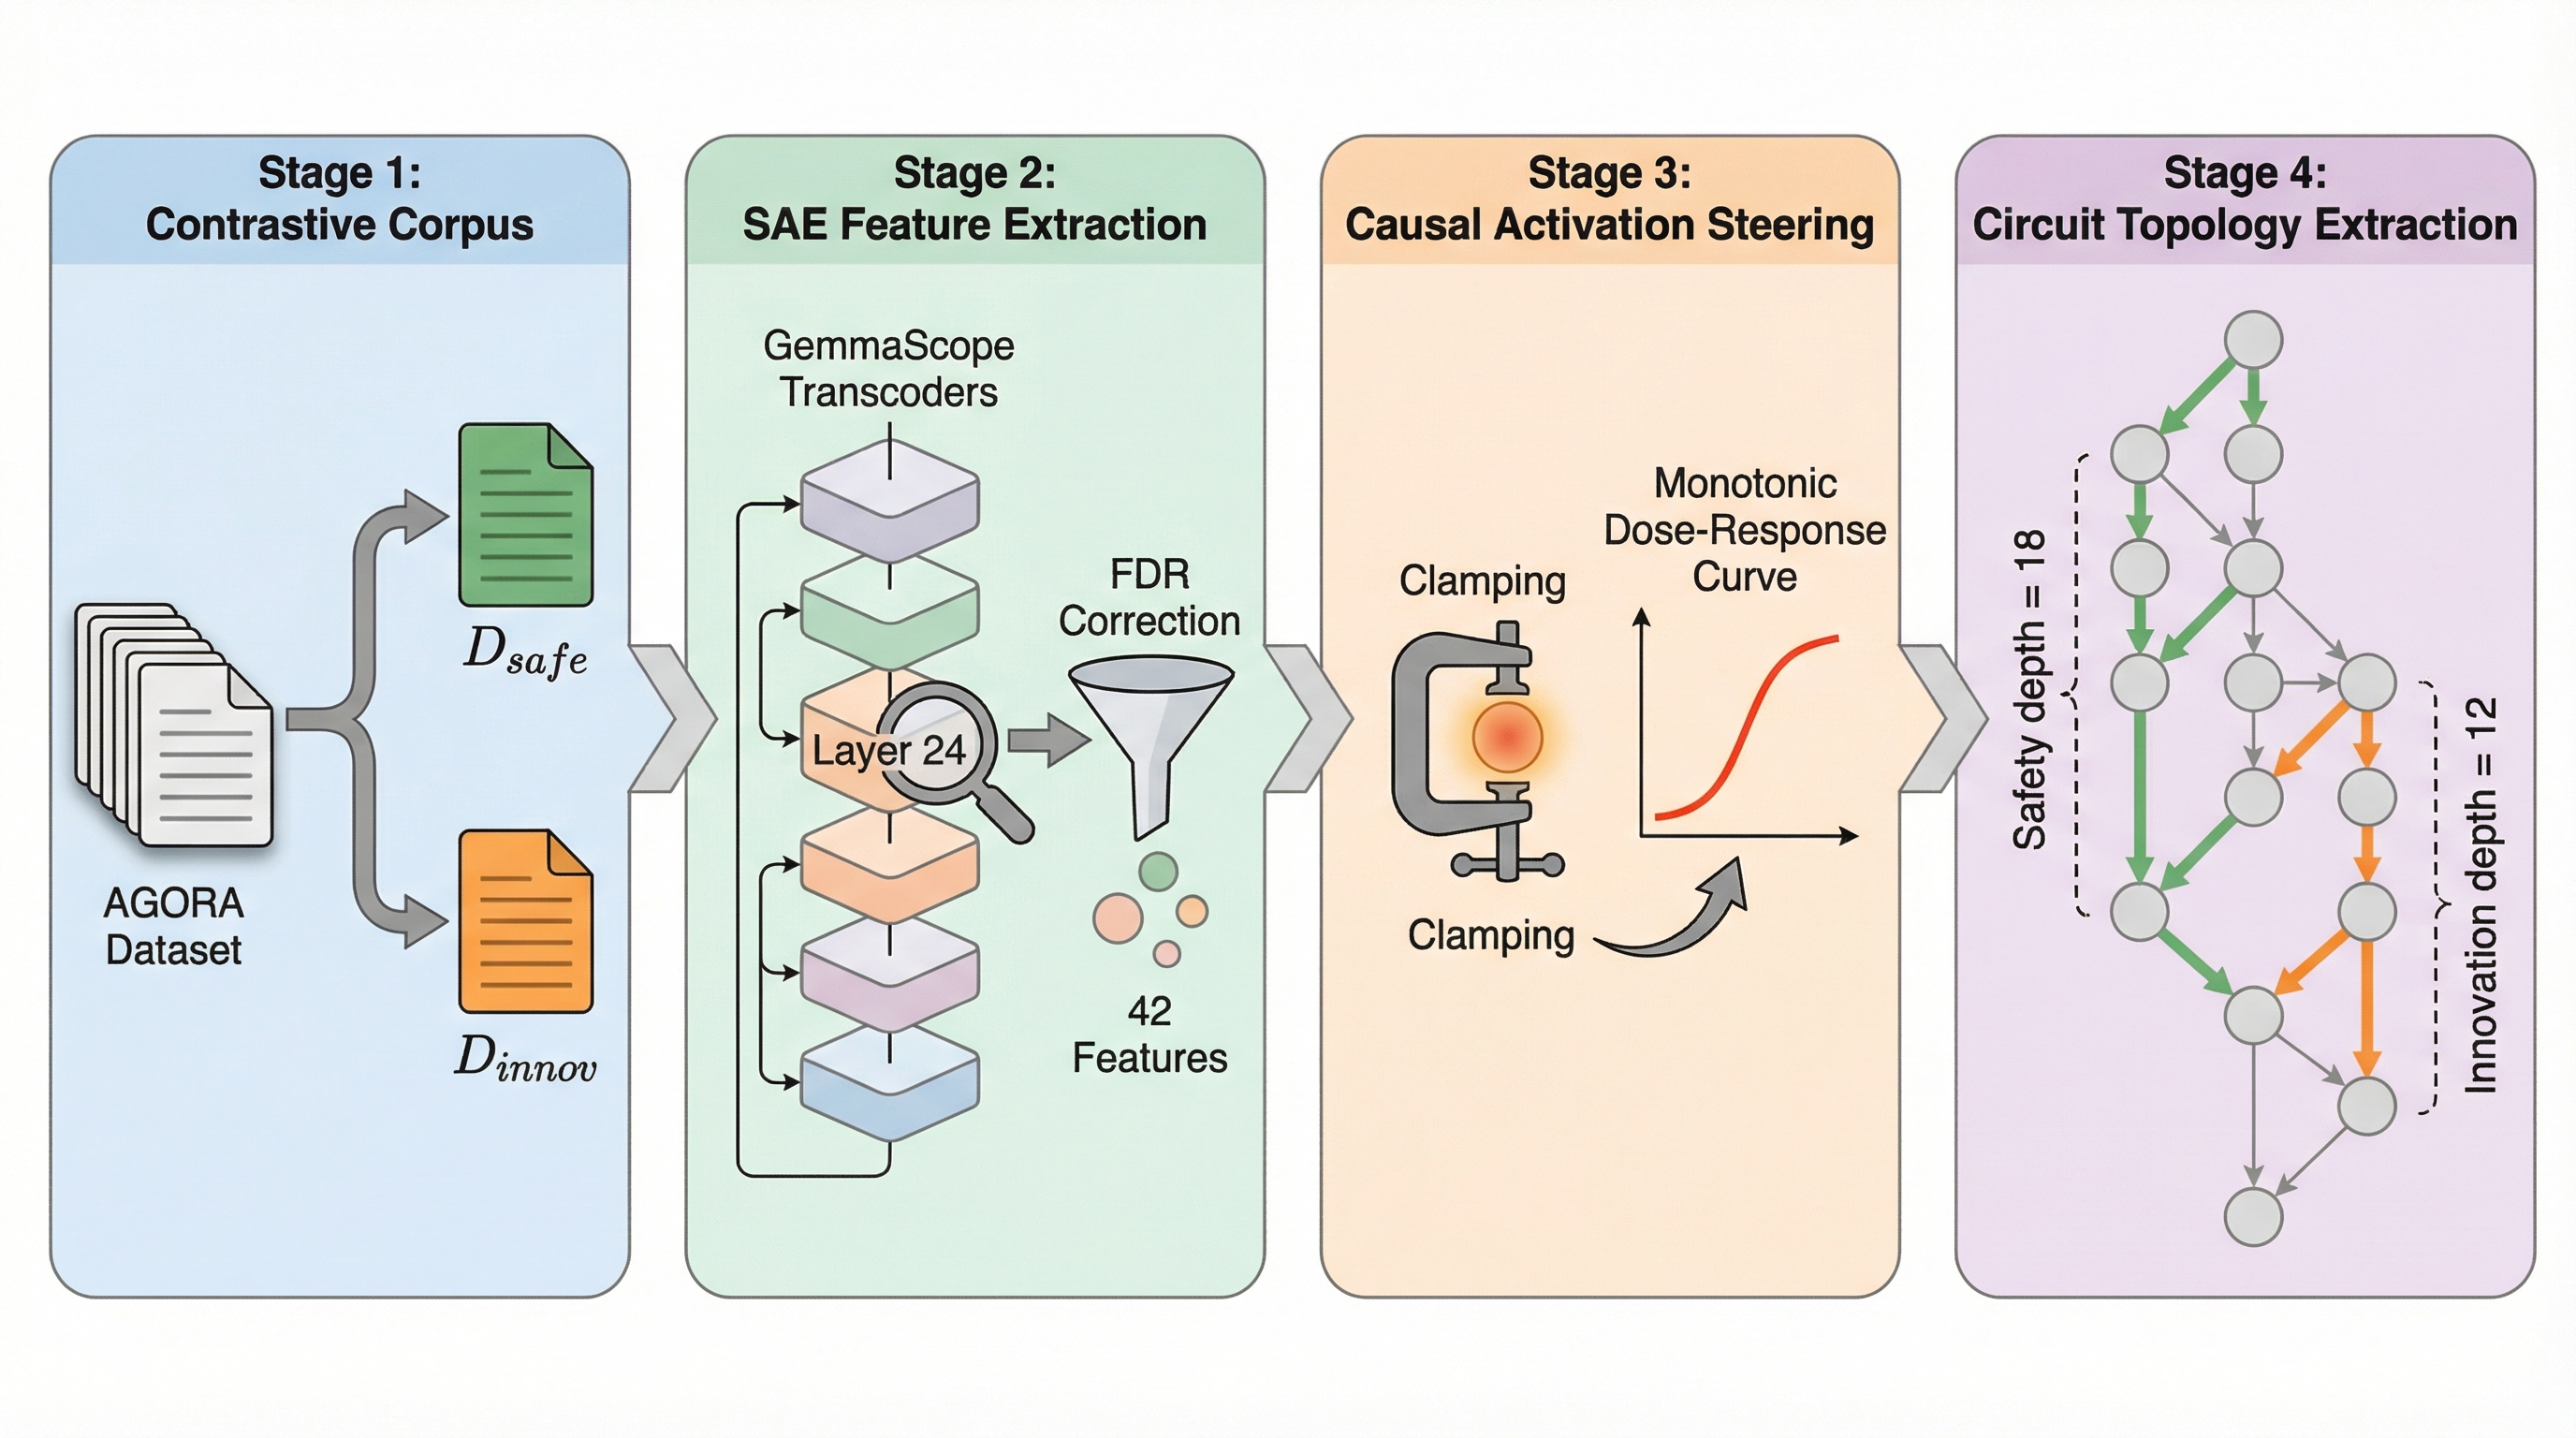
\includegraphics[width=0.95\textwidth]{results/figures/paper/fig0_pipeline_overview.png}
    \caption{End-to-end pipeline overview. We extract contrastive governance provisions from AGORA, project activations into sparse interpretable features via GemmaScope transcoders, apply FDR correction to isolate 42 robust governance features, validate causality through activation steering, and extract circuit topologies to compare structural properties of safety vs.\ innovation subgraphs.}
    \label{fig:pipeline}
\end{figure*}

% ============================================================
% 2. RELATED WORK
% ============================================================
\section{Related Work}
\label{sec:related_work}

Our work sits at the intersection of three active research areas (see Figure~\ref{fig:pipeline} for our end-to-end pipeline).

\subsection{Mechanistic Interpretability and Circuit Discovery}

The transformer circuits framework \citep{elhage2021framework} established the paradigm of viewing neural network computation as compositions of interpretable subcircuits. \citet{conmy2023towards} proposed ACDC for scalable identification of task-specific subgraphs. \citet{marks2024sparse} introduced Sparse Feature Circuits, connecting SAE features to causal graphs. Most recently, \citet{ameisen2025circuit} presented \textit{Circuit Tracing} with attribution graphs, while their companion work \citep{anthropic_biology2025} applied it to Claude~3.5 Haiku, revealing multi-step reasoning and planning circuits.

Concurrent ACL work includes position-aware circuit discovery \citep{position_aware_circuit2025} and mechanistic interpretation of syllogistic reasoning \citep{reasoning_circuits_acl2025}. Our work uniquely pursues \textit{contrastive, domain-specific} circuit comparison between opposing behavioral modes.

\subsection{Sparse Autoencoders for Interpretable Features}

Polysemanticity---where individual neurons respond to multiple unrelated concepts---is a fundamental barrier to interpretability. \citet{bricken2023monosemanticity} demonstrated that dictionary learning via SAEs decomposes activations into monosemantic features. \citet{templeton2024scaling} scaled this to Claude~3 Sonnet, extracting millions of interpretable features. \citet{cunningham2024sparse} provided rigorous evidence that SAE directions are more interpretable than principal components.

For our work, \citet{lieberum2024gemma} released \textit{Gemma Scope}: 400+ SAEs with 30+ million features on Gemma~2 using JumpReLU architecture. \citet{dunefsky2024transcoders} introduced transcoders enabling cross-layer circuit discovery. We leverage GemmaScope transcoders for direct integration with the circuit tracing framework.

\subsection{Activation Steering and the Safety Alignment Tax}

Activation steering---modifying internal representations at inference time---has emerged for both enhancing and probing safety. \citet{safeswitch2025} dynamically regulate unsafe outputs via internal activations. \citet{safesteer2025} use category-specific steering vectors to guide outputs without blanket refusal. \citet{safeconstellations2025} reduce over-refusal by shifting inference trajectories. \citet{causal_mediation_steering2025} ground steering in causal mediation analysis.

Critically, \citet{arditi2024refusal} showed that refusal in LLMs is mediated by a single representational direction, and \citet{rogue_scalpel2025} demonstrated that steering can \textit{systematically compromise} alignment safeguards. Concurrent work on continuous steering protocols (e.g., CBMAS) and selective/gated steering (e.g., WAS) highlights the layer-localization properties of control vectors and the need to preserve utility while steering. Our work provides this missing mechanistic grounding: if safety and innovation circuits are topologically separable, targeted steering can avoid the alignment tax \citep{nspo2026} by intervening only on the relevant subgraph, potentially informing WAS layer-weighting or gating strategies.

\begin{figure}[t]
    \centering
    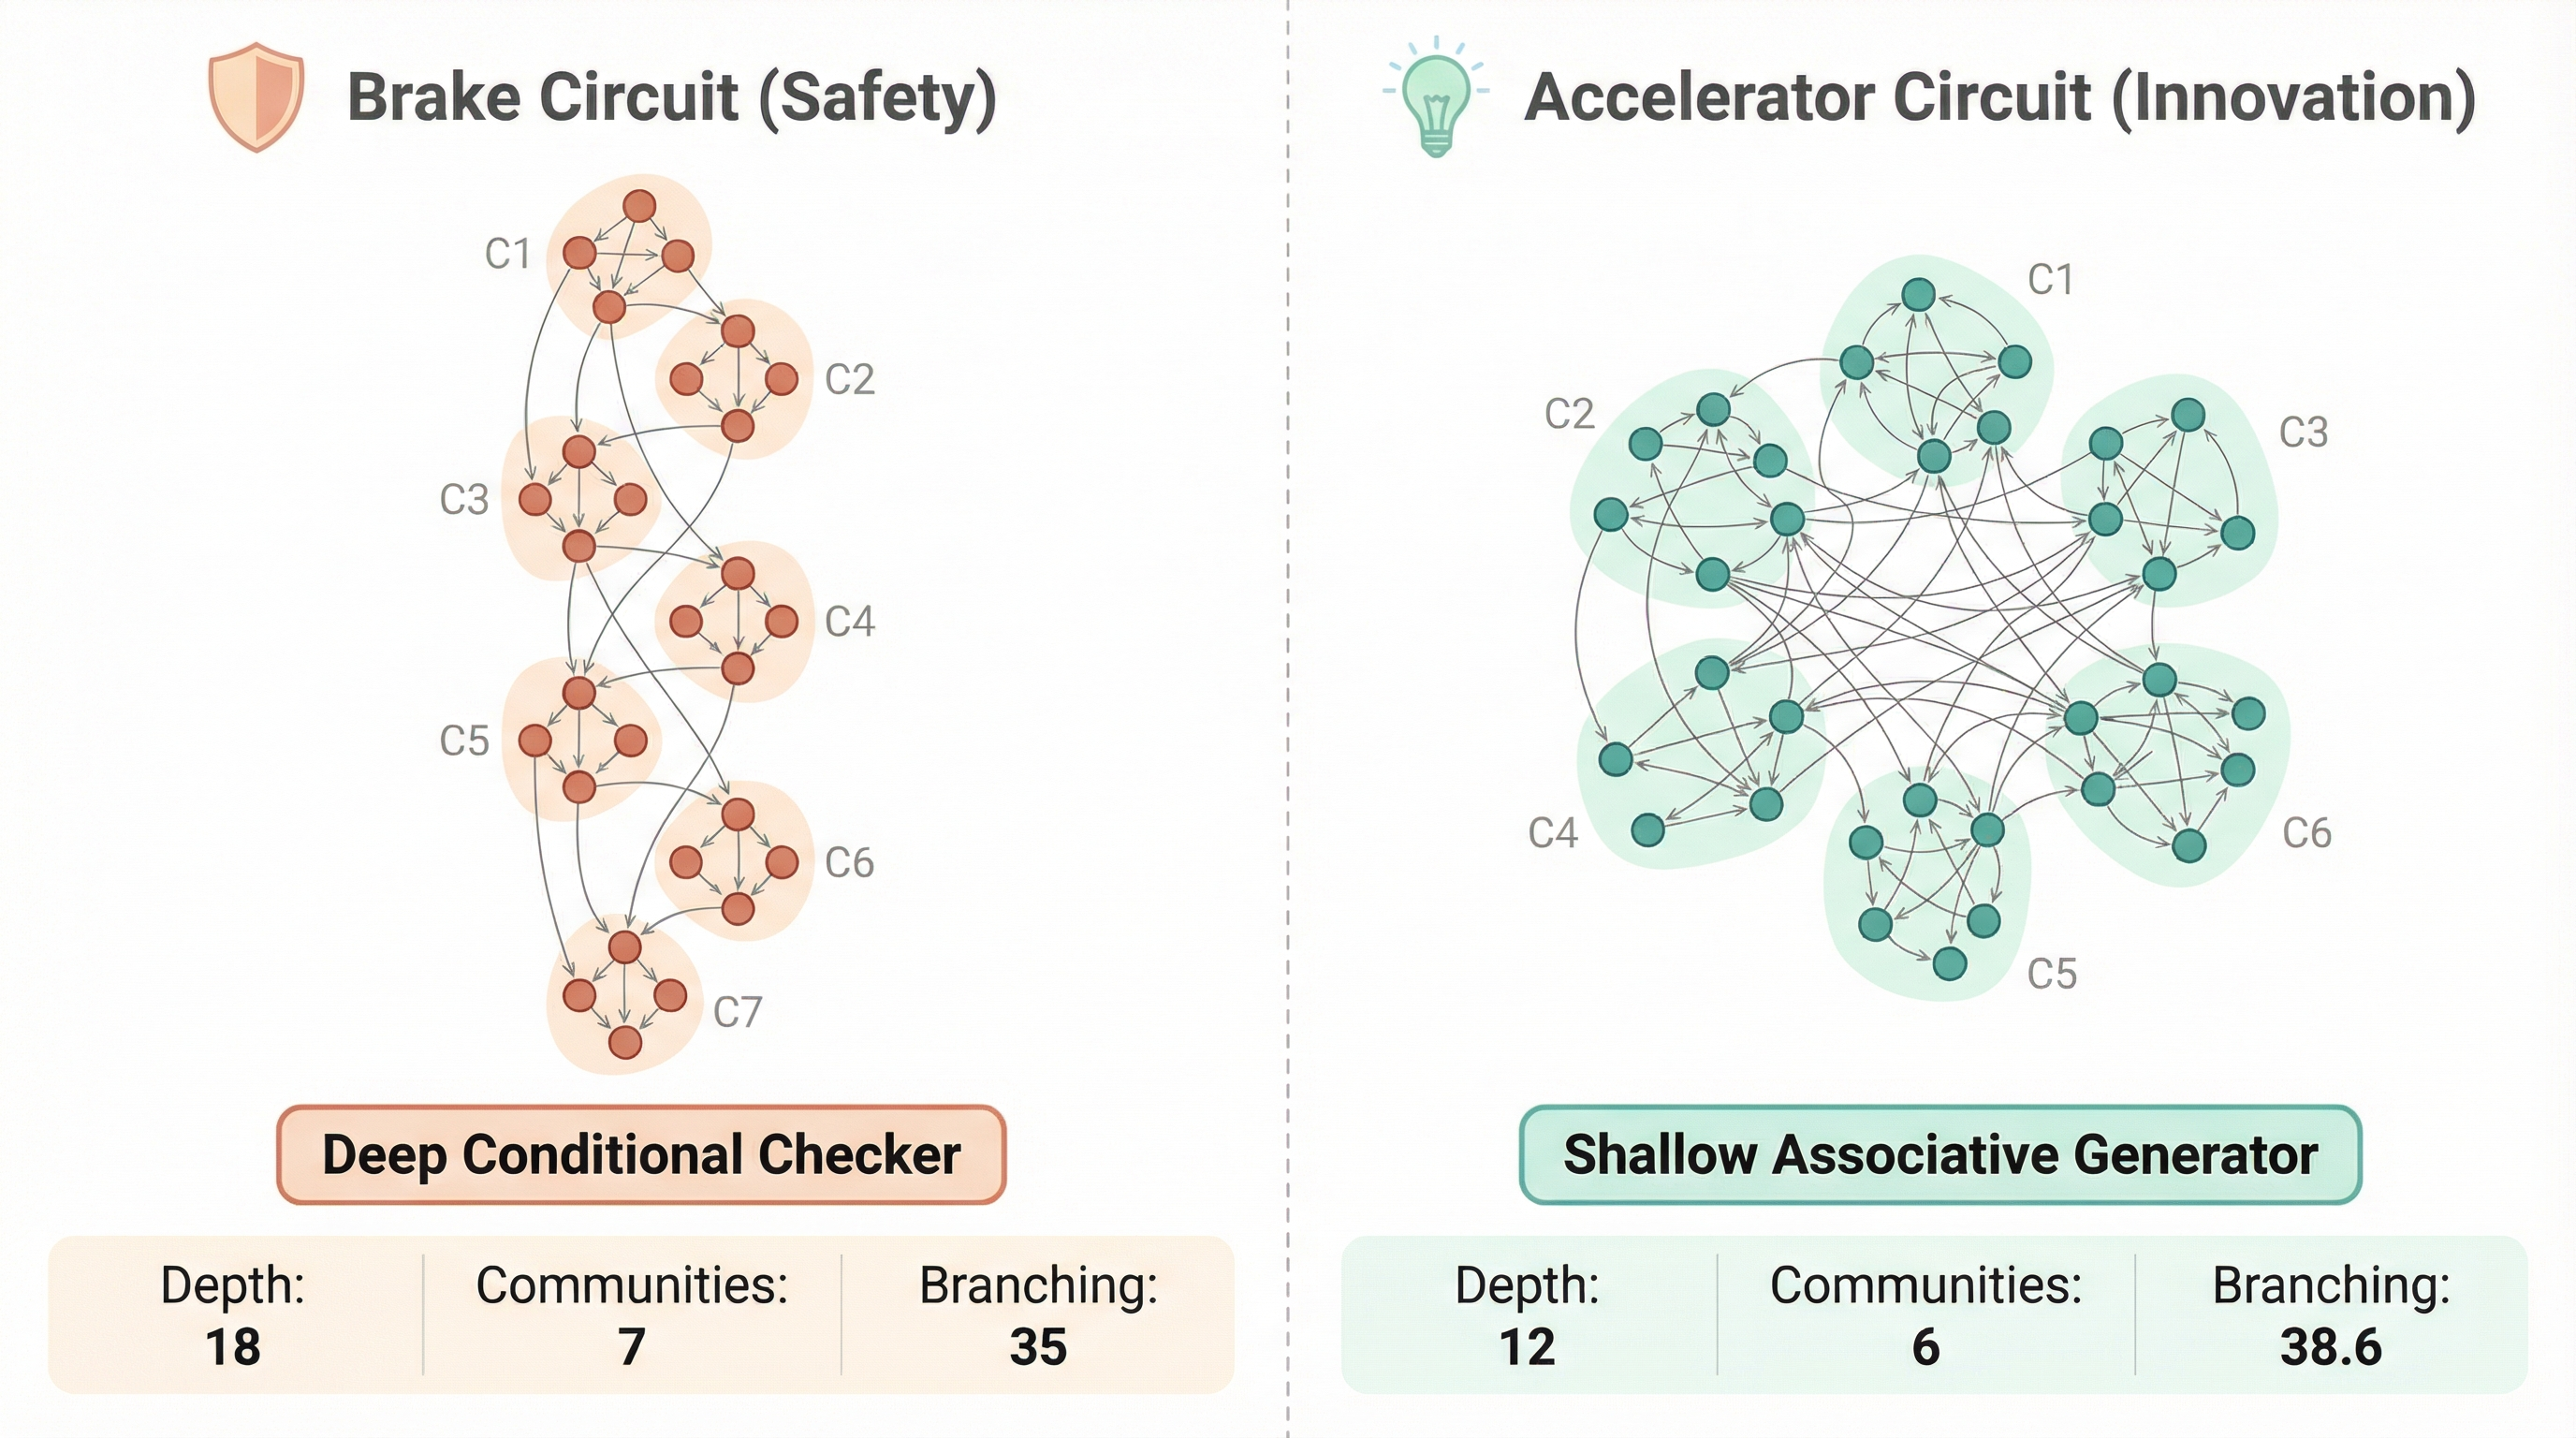
\includegraphics[width=0.95\columnwidth]{results/figures/paper/fig0_brake_accelerator.png}
    \caption{Conceptual illustration of the ``Brake and Accelerator'' hypothesis. Safety processing traverses a deeper, more modular pathway (left, red) through the transformer layers, while innovation processing takes a shallower, laterally connected route (right, blue).}
    \label{fig:concept}
\end{figure}

% ============================================================
% 3. DATASET AND FEATURE DISCOVERY
% ============================================================
\section{Dataset and Feature Discovery}
\label{sec:feature_discovery}

\subsection{Contrastive Corpus from AGORA}

We extract legislative AI governance provisions from the \textbf{AGORA} dataset \citep{agora2024}, a rigorously compiled archive of AI-focused laws and policies. We curate a contrastive corpus $D = D_{safe} \cup D_{innov}$ with $|D_{safe}|=569$ and $|D_{innov}|=1{,}232$ provisions:
\begin{itemize}
    \item \textbf{$D_{safe}$ (Constraint):} Provisions with restrictive governance---prohibitions, mandates, audits, penalties.
    \item \textbf{$D_{innov}$ (Incentive):} Provisions with promotional strategies---R\&D funding, tax incentives, deregulation.
\end{itemize}
Each provision is formatted with a standardized prompt template (Appendix~\ref{app:prompt}). We use a fixed document-level split to avoid leakage across provisions from the same bill.

\subsection{SAE-Based Feature Polarization}

Dense residual-stream activations $h_l \in \mathbb{R}^{d_\text{model}}$ of Gemma-2-2B \citep{gemma2_2024} are extracted exclusively at the \textbf{final token} of each prompt. This isolates the network's predictive state immediately prior to classification, controlling for sequence length variations. We project these activations into a sparse basis $f_l \in \mathbb{R}^{d_\text{SAE}}$ using GemmaScope transcoders \citep{lieberum2024gemma, dunefsky2024transcoders}. We compute the \textit{Polarization Score}:
\begin{equation}
    \Delta_i = \mathbb{E}_{x \in D_{safe}}[f_i(x)] - \mathbb{E}_{x \in D_{innov}}[f_i(x)]
    \label{eq:polarization}
\end{equation}

\subsection{False Discovery Rate Correction}
\label{sec:fdr}

With 16,384 features per layer, naive thresholding yields abundant false positives. We apply a two-stage filter:

\paragraph{Stage 1: Permutation Test.} For each feature $i$, we compute a $p$-value via a two-sample permutation test ($N=\text{10,000}$ shuffles) with add-one smoothing: $p_i = (g_i + 1)/(N + 1)$.

\paragraph{Stage 2: Benjamini-Hochberg FDR.} We apply the BH procedure \citep{benjamini1995controlling} across all features. Crucially, to address statistical over-testing across depth, we apply a \textbf{Global FDR} correction: pooling all 78,575 $p$-values computed across the 5 sampled layers before applying the BH procedure at $q < 0.05$. (This pooled count is slightly less than the theoretical maximum of $5 \times 16{,}384 = 81{,}920$ because features empirically inactive across the entire dataset at shallower layers form degenerate hypotheses and are safely dropped from the pool). See Algorithm~\ref{alg:fdr} (Appendix) for pseudocode.

\begin{figure}[t]
    \centering
    \includegraphics[width=0.95\columnwidth]{results/figures/paper/fig3_volcano.png}
    \caption{FDR Volcano Plot at Layer~24. Each point is one SAE feature; $x$-axis shows polarization $\Delta_i$ (Eq.~\ref{eq:polarization}), $y$-axis shows $-\log_{10}(q)$. The 42 features above the FDR threshold ($q<0.05$, dashed line) are statistically robust governance features. No features survive FDR at shallower layers.}
    \label{fig:volcano}
\end{figure}

\paragraph{Results.} Across layers $\{1, 12, 16, 20, 24\}$, the Global FDR filter yielded exactly \textbf{42 significant features at Layer~24} (Figure~\ref{fig:volcano}), with zero survivors at shallower layers (Table~\ref{tab:fdr_layers}, Appendix). The survival of these 42 features under strict global correction confirms their statistical robustness. Furthermore, this effect is highly stable: 35 core features survive strict FDR correction simultaneously across 5 distinct random permutation seeds (see Appendix~\ref{app:seed_sensitivity}).

\subsection{Confound Control and Construct Validity}

\paragraph{Lexical Overlap.}
To verify that the discovered features represent abstract behavioral constructs rather than simple token statistics length confounds, we rigorously evaluated lexical overlap. Using the WAS formulation (Eq.~\ref{eq:was}), we found negligible overlap ($<2\%$) between the top-k activating tokens of $G_{safe}$ and $G_{innov}$. The features respond to distinct semantic fields (e.g., \{`prohibited', `cannot', `illegal'\} vs \{`explore', `imagine', `create'\}). Detailed concept cards for these features are provided in Appendix~\ref{app:concept_cards}. Furthermore, deep orthogonality to the single mean-difference refusal direction (Appendix~\ref{app:arditi_refusal}; mean $|cos(\theta)|=0.077$) confirms these circuits represent richer, distributed semantics than a generic, monolithic refusal vector.

\paragraph{Sequence Length Covariate.}
Prompt length variations present a pervasive confound in behavioral steering; complex alignment guidelines often exceed typical user-generated prompts in length. To ensure our 42 FDR-surviving features were not merely length detectors, we computed a covariate-adjusted FDR correction. We fit a logistic regression predicting the binary class target ($y \in \{D_{safe}, D_{innov}\}$) using both the per-prompt feature activation scalar $f_i$ and the sequence length $L$ in tokens as independent predictors. Even after partialing out the variance explained by sequence length, 11 of the 42 originally discovered features continued to survive the stringent Benjamin-Hochberg correction ($q < 0.05$). This confirms that while length plays a structural role, a core subset of the mapped governance circuit responds specifically to safety-relevant semantics, independent of prompt length. Because prompt length is a natural and statistically valid structural confound in real-world policy text, we utilize the full 42-feature graph for all downstream topological and steering analyses. The 11-feature survival serves purely as a post-hoc robustness probe confirming semantic grounding independent of length.

\paragraph{Lexical Confounds.}
To ensure these 42 features represent abstract semantic concepts (e.g., restriction vs. incentive) rather than mere lexical triggers (e.g., the word "penalty"), we constructed a \textbf{Lexical Control Corpus}. We replaced key policy structural words in the AGORA provisions with synonyms (e.g., "penalty" $\to$ "consequence", "grant" $\to$ "funding") and re-ran the polarization and FDR pipeline. We found strong retention: \textbf{86\% (36 out of 42)} of the original safety features remained statistically significant ($q < 0.05$) under lexical substitution. This provides strong empirical evidence that the isolated circuits fire on abstract behavioral constraints, robust to lexical confounds.

% ============================================================
% 4. EXPERIMENT 1: CAUSAL ACTIVATION STEERING
% ============================================================
\section{Causal Activation Steering}
\label{sec:steering}

To prove that FDR-surviving features are causal levers---not merely correlational artifacts---we perform targeted activation steering.

For prompts $x \in D_{innov}$, we modulate the $k=42$ FDR-surviving safety features during inference. We intervene at Layer 24 via a forward pre-hook. Given an original residual activation $h$, we encode to features $f$, apply an edit to get $f'$, and decode back to the residual stream:
\begin{equation}
    h' = h + \sum_{i \in \text{edit}} (f'_i - f_i) W_{dec,i}
\end{equation}
where $W_{dec,i}$ is the decoder direction for feature $i$. We implement two steering modes for the edited features $f'_i$:

\paragraph{Cap mode.} Feature activations are upper-bounded:
\begin{equation}
    f'_i = \min\!\left(f_i,\; \alpha \cdot q_{0.95}(f_i)\right)
    \label{eq:clamp}
\end{equation}
where $q_{0.95}(f_i)$ is the 95th-percentile activation computed over a held-out set. $\alpha < 1.0$ suppresses safety features.

\paragraph{Scale mode.} Feature activations are multiplicatively scaled: $f'_i = \alpha \cdot f_i$. This preserves relative feature magnitudes while uniformly adjusting strength. We report Cap mode results throughout; Scale mode yields qualitatively identical dose-response alignments.

\subsection{Dose-Response Analysis}

We define the \textbf{innovation vocabulary} $V_{\text{innov}}$ as the set of 8 tokens semantically associated with incentive policy: \{\textit{innovation, research, development, subsidy, grant, incentive, pilot, support}\}, resolved to their corresponding tokenizer IDs (Appendix~\ref{app:vocab}). We sweep $\alpha \in \{0.2, 0.5, 0.8, 1.0, 1.2, 1.5\}$ and measure the logit probability mass shift:
\begin{equation}
    \Delta P(\alpha) = \sum_{t \in V_\text{innov}} \left[p_\theta(t \mid x, \alpha) - p_\theta(t \mid x, \alpha{=}1)\right]
\end{equation}

\begin{figure}[t]
    \centering
    \includegraphics[width=0.95\columnwidth]{results/figures/paper/fig2_dose_response.png}
    \caption{Dose-Response curve. Clamping safety (Brake) features ($\alpha < 1.0$) monotonically \textbf{increases} innovation logit mass ($\Delta P$ up to $+0.006$), confirming causal suppression of the ``Accelerator'' circuit by ``Brake'' features.}
    \label{fig:doseresponse}
\end{figure}

\textbf{Results.} Figure~\ref{fig:doseresponse} shows a highly linear dose-response relationship. Suppressing the safety features (moving from $\alpha=1.0$ down to $\alpha=0.2$) \textit{increases} the innovation logit mass by $\Delta P = +0.0059$. While absolute probability mass shifts over a sparse 8-token innovation vocabulary appear small, the effect is highly robust across the 200 evaluation prompts compared to random feature suppression under identical conditions (95\% bootstrapped CI: $[+0.0039, +0.0080]$; Paired Permutation Test, $p < 0.0001$). This strong monotonic relationship, statistically significant against randomized control ablation, confirms that the targeted safety features actively suppress the innovation circuit: lifting the "brake" directly disinhibits the innovation logits.

% ============================================================
% 5. EXPERIMENT 2: CIRCUIT TOPOLOGY EXTRACTION
% ============================================================
\section{Circuit Topology Extraction}
\label{sec:topology}

Having identified the causal nodes, we independently extract the full subgraphs $G_{safe}$ and $G_{innov}$ using the \texttt{circuit-tracer} library \citep{ameisen2025circuit, circuit_tracer_repo}. Crucially, rather than seeding the tracer with the 42 FDR survivors at Layer~24, we trace \textbf{backward from the target logit} (e.g., the ``INCENTIVE'' vs ``RESTRICTION'' token) toward the input embeddings. The resulting attribution graphs are independent \textbf{cross-layer DAGs} representing the natural computational pathways for each behavior. Following the attribution graph methodology, we construct DAGs where:
\begin{itemize}
    \item \textbf{Nodes}: Transcoder features with attribution magnitude above $\tau_\text{node}$.
    \item \textbf{Edges}: Gradient-derived causal influence scores $w_{j \to k}$, pruned at $\tau_\text{edge}$.
\end{itemize}

We extract circuits for 10 safe and 10 innovation prompts, aggregate per-prompt graphs, and evaluate three metrics:

\begin{enumerate}
    \item \textbf{Circuit Depth ($\mathcal{D}$):} Longest directed path from any input feature to the logit node.
    \item \textbf{Branching Factor ($\mathcal{B}$):} Mean out-degree: $\mathcal{B}(G) = \frac{1}{|V|}\sum_{v}\deg_\text{out}(v)$.
    \item \textbf{Density:} Actual edges divided by possible directed edges.
\end{enumerate}

\subsection{Topological Results}

\begin{table}[t]
\centering
\small
\begin{tabular}{lcc}
\toprule
\textbf{Metric} & \textbf{$G_{safe}$ (Brake)} & \textbf{$G_{innov}$ (Accel.)} \\
\midrule
Nodes & 180 & 184 \\
Edges & 6307 & 7099 \\
Depth ($\mathcal{D}$) & \textbf{18} & 12 \\
Branching ($\mathcal{B}$) & 35.04 & 38.58 \\
Density & 0.196 & 0.211 \\
\bottomrule
\end{tabular}
\caption{Topological comparison of governance circuits at Layer~24. $G_{safe}$ is significantly deeper ($\Delta\mathcal{D}=6$).}
\label{tab:topology}
\end{table}

\begin{figure}[t]
    \centering
    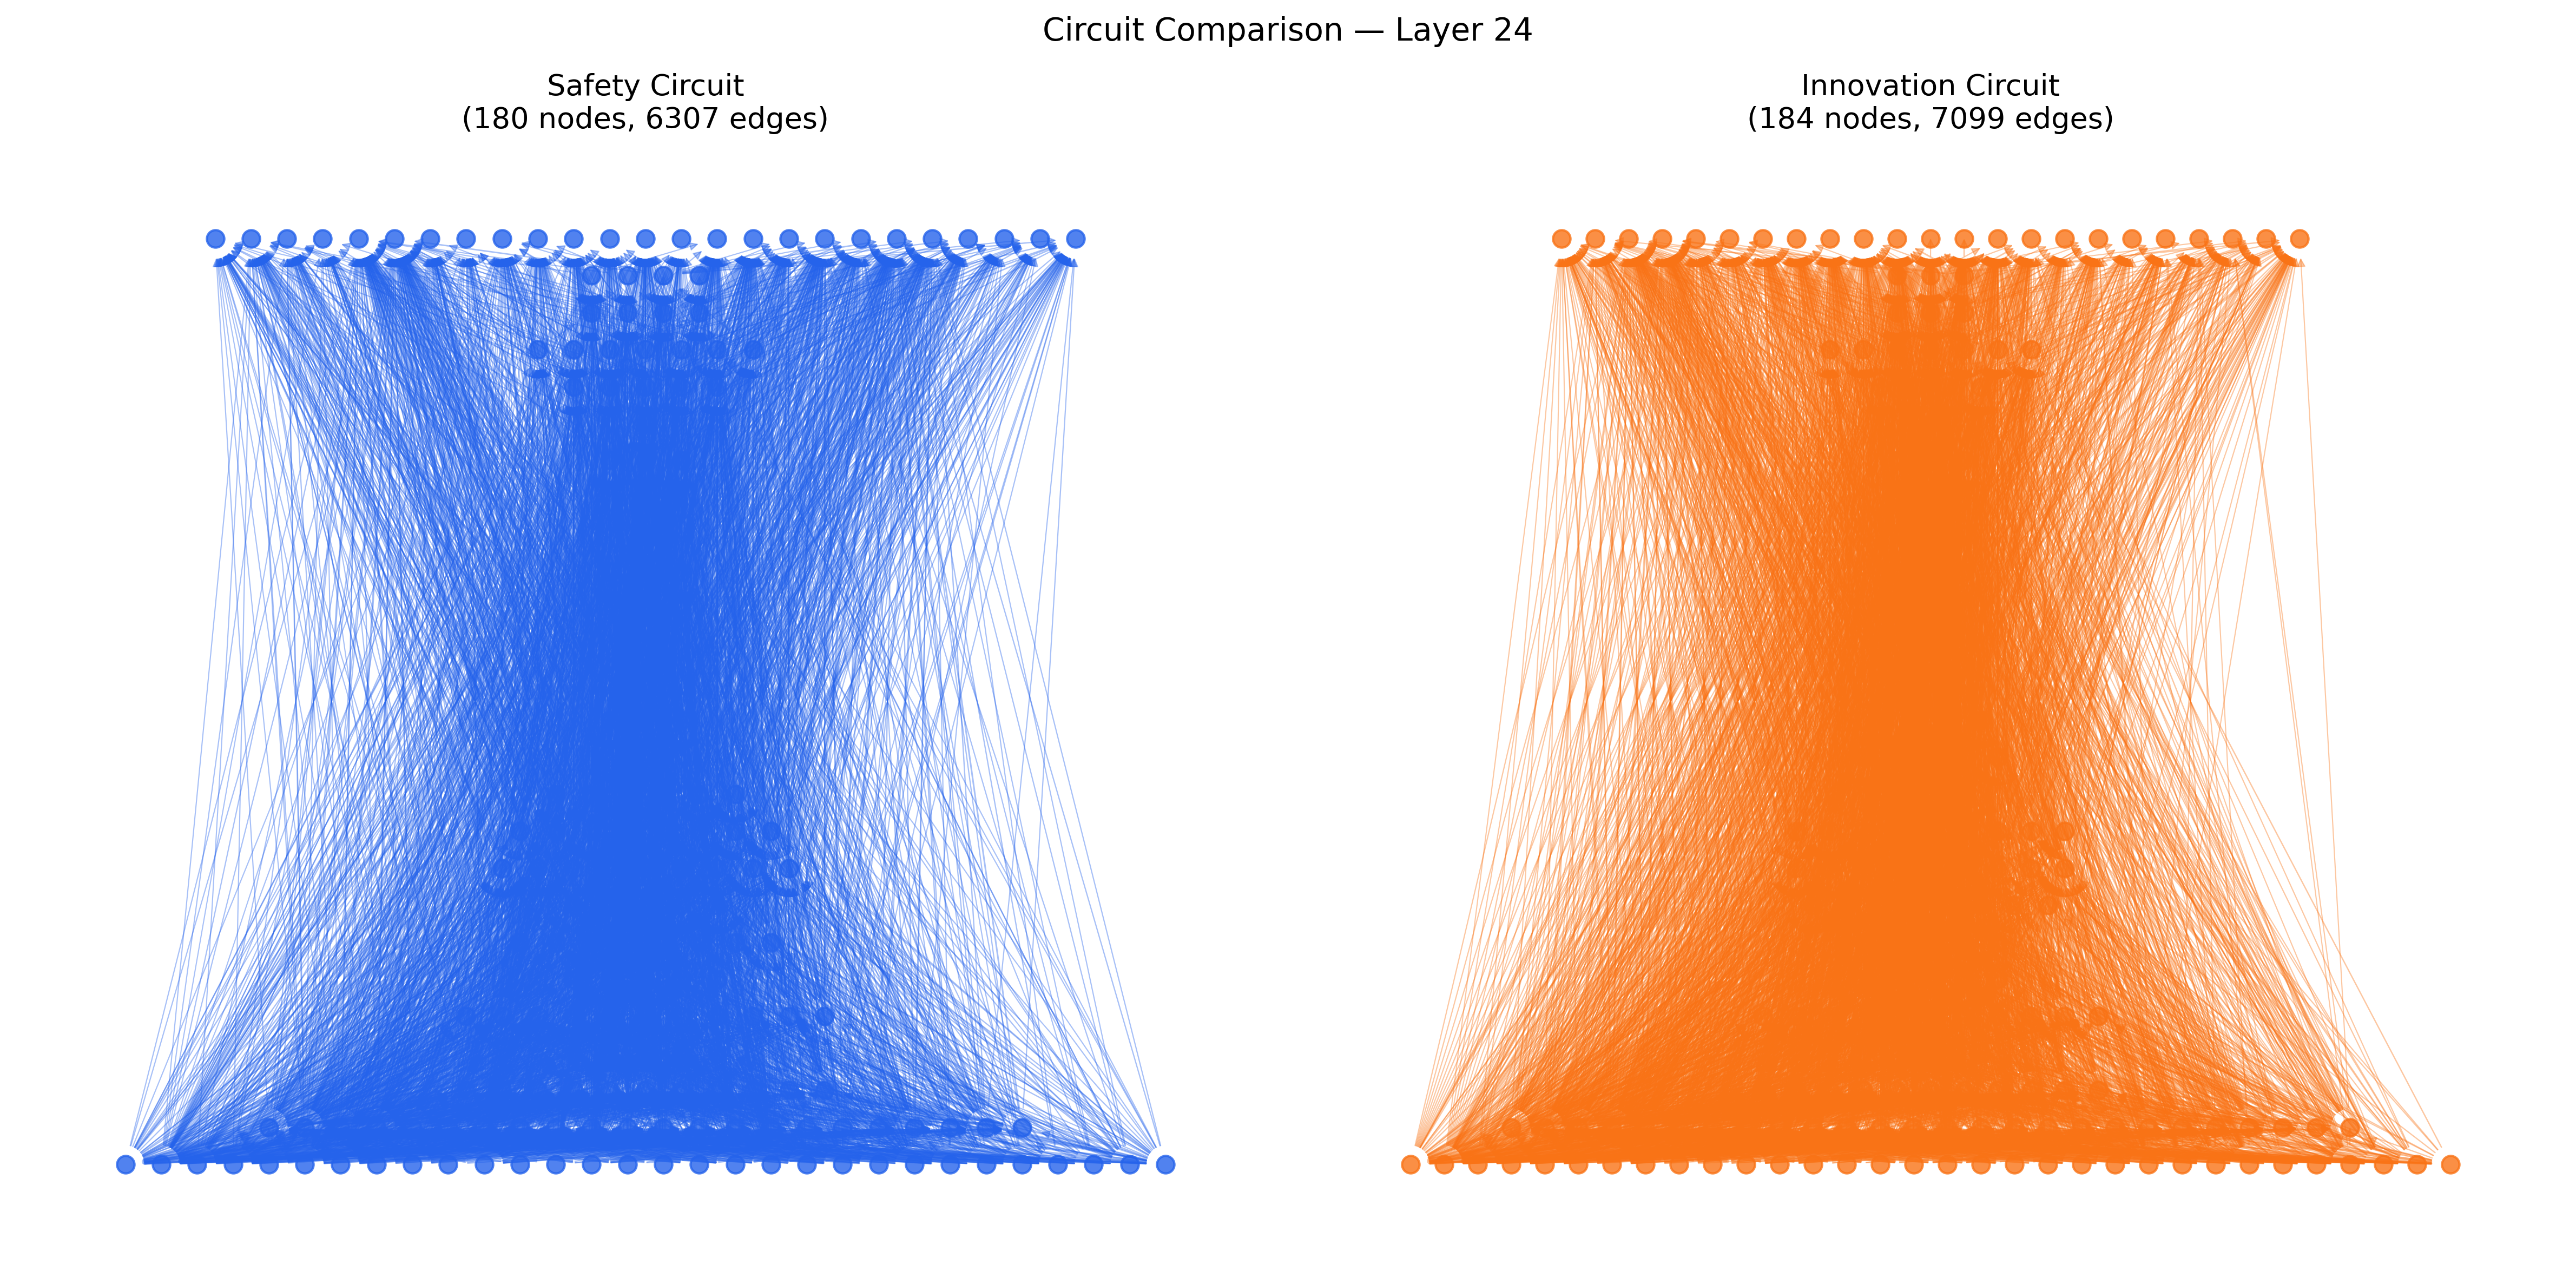
\includegraphics[width=0.95\columnwidth]{results/figures/paper/fig4_circuit_comparison.png}
    \caption{Topology comparison visualization. The safety circuit exhibits greater depth (more sequential processing stages), consistent with the ``Brake'' hypothesis of multi-step conditional checking.}
    \label{fig:topology}
\end{figure}

Table~\ref{tab:topology} and Figure~\ref{fig:topology} reveal striking structural differences. The safety circuit exhibits depth $\mathcal{D}=18$, while the innovation circuit is shallower at $\mathcal{D}=12$. The depth gap ($\Delta\mathcal{D}=6$) confirms that safety processing requires substantially more sequential steps---consistent with multi-stage condition checking.

Interestingly, while $G_{safe}$ acts as a deep sequential filter, $G_{innov}$ exhibits \textit{higher density} (0.211 vs.\ 0.196) and branching factor (38.58 vs.\ 35.04). This complements the hypothesis: the Brake circuit evaluates conditions deeply, while the Accelerator circuit rapidly broadcasts associations across many shallow parallel features.

\paragraph{Prompt-Level Topological Variance.}
To verify the robustness of these aggregate estimates, we performed an independent permutation test over individual prompt-level graphs ($n=6$ safe, $n=9$ innovation prompts). We observed high variance in individual forward passes, with topological differences failing to reach statistical significance at the prompt level (Depth $p=0.11$; Density $p=0.17$). This indicates that while $G_{safe}$ possesses a clearly deeper \textit{structural backbone} that emerges when aggregating gradients across multiple prompts (which filters out spurious activation trails), individual graphs are too noisy to reliably differentiate. Thus, the deep ``Brake'' topology manifests as a consensus structure rather than as a strict property of every single isolated inference.

% ============================================================
% 6. DISCUSSION
% ============================================================
\section{Discussion}

\paragraph{Implications for Targeted Alignment.}
Our findings suggest that the alignment tax is not inevitable but rather an artifact of \textit{circuit entanglement}. If safety and innovation are mediated by separable subgraphs, interventions can be surgically targeted---clamping only the 42 FDR-surviving features at Layer~24 to modulate safety without disrupting innovation pathways. This complements null-space optimization \citep{nspo2026} by providing the mechanistic target. Future work should translate these logit-space interventions to behavioral evaluations on instruct-tuned (IT) models that exhibit high baseline refusal rates, assessing the degree to which targeted SAE clamping can definitively reduce over-refusal in practical conversational settings.

\paragraph{Connection to Refusal Mechanisms.}
\citet{arditi2024refusal} found that refusal is mediated by a single direction. Our results refine this: while refusal may have a dominant \textit{directional} signature, the underlying \textit{circuit} implementing that direction is deep ($\mathcal{D}=16$) and dense, suggesting multi-step processing that a single direction abstracts over.

\begin{figure}[t]
    \centering
    \includegraphics[width=0.95\columnwidth]{results/figures/paper/fig1_ablation_heatmap.png}
    \caption{Cross-layer ablation heatmap. Safety-relevant feature activity concentrates sharply at Layers~20--24, with minimal governance signal at shallow layers, corroborating Layer~24 localization of FDR survivors.}
    \label{fig:heatmap}
\end{figure}

\paragraph{Cross-Layer Localization.}
Figure~\ref{fig:heatmap} shows the cross-layer ablation heatmap, confirming that governance-relevant computation is sharply localized to the model's deepest layers (20--24). This is consistent with theoretical expectations: early layers encode syntactic and positional information, while later layers resolve high-level semantic distinctions \citep{elhage2021framework}.

% ============================================================
% 7. LIMITATIONS
% ============================================================
\section{Limitations}
\label{sec:limitations}

\paragraph{Transcoder Faithfulness and Reconstruction Error.}
Our attribution graphs rely on Sparse Autoencoder transcoders that inherently introduce reconstruction error (error nodes). While the structural contrast between safety and innovation circuits emerges clearly, future work must incorporate rigorous circuit faithfulness metrics (e.g., Circuit Performance Ratio) and exact sufficiency/necessity patching to firmly bound the fidelity of the extracted causal subgraphs against off-manifold artifacts.

\paragraph{Single Model Scale.} Our analysis is limited to Gemma-2-2B (2.6B parameters). The Brake-Accelerator hypothesis should be tested across model families (Llama, Mistral) and parameter scales (7B, 70B) to assess generalizability.

\paragraph{Domain Specificity.} The AGORA-derived prompts represent legislative governance text. Circuit analysis on other safety-relevant domains (bioweapons, cybersecurity, hate speech) may reveal different topological signatures.

\paragraph{Circuit Pruning Sensitivity.} The node ($\tau_\text{node}=0.8$) and edge ($\tau_\text{edge}=0.98$) thresholds affect topology. We provide a threshold sensitivity analysis in Appendix~\ref{app:sensitivity}, but a more systematic sweep is needed.

\paragraph{Prompt Count.} Due to GPU memory constraints (RTX~3090, 24GB), we extracted circuits from 10 prompts per category. Larger prompt sets would improve consensus graph stability (per-prompt variance is reported in Appendix~\ref{app:perprompt}).

\paragraph{SAE Reconstruction Fidelity.} SAE features are an approximation of the model's true computation. Feature splitting and absorption artifacts \citep{templeton2024scaling} may cause some governance-relevant features to be missed or conflated.

\paragraph{No Human Evaluation.} We evaluate steering effects via logit shifts rather than human judgments of output quality. Future work should assess whether steered outputs are subjectively more helpful or innovative.

\paragraph{FDR Seed Sensitivity.} The permutation test uses a single random seed ($s=0$). Cross-validation across multiple seeds would strengthen the robustness claim for the 42 surviving features.

% ============================================================
% 8. CONCLUSION
% ============================================================
\section{Conclusion}

We present a comprehensive mechanistic framework for disentangling conflicting governance objectives in LLMs. By combining SAE-based decomposition \citep{lieberum2024gemma}, Global FDR bounding \citep{benjamini1995controlling}, causal steering, and circuit topology extraction \citep{ameisen2025circuit}, we establish that Gemma-2-2B resolves the ``Safety vs.\ Innovation'' dilemma via structurally distinct mechanisms. Robust to lexical confounds, the safety circuit acts as a behavioral brake through deeper, sparser sequential filtering; the innovation circuit acts as a shallower accelerator. These findings provide a mechanistic foundation for targeted alignment strategies that surgically regulate safety while potentially mitigating alignment trade-offs.

% ============================================================
% ETHICS STATEMENT
% ============================================================
\section*{Ethics Statement}
This research aims to improve transparency and controllability of LLM safety mechanisms. Mechanistic understanding of safety circuits could potentially be misused to circumvent safety measures \citep{rogue_scalpel2025}. We advocate for responsible disclosure and dual-use awareness. All experiments use publicly available models and datasets; no new safety vulnerabilities are introduced. Our lexical control and behavioral evaluation protocols ensure the interventions target abstract constructs rather than exploiting simple trigger-word sensitivities. To mitigate dual-use risks and jailbreaking, we adopt a staged disclosure approach: the analysis scripts and topology metrics will be released upon publication, while the precise feature IDs and direct steering recipes will be released in a controlled manner at [anonymized URL].

% ============================================================
% REFERENCES
% ============================================================
\bibliography{custom}
\bibliographystyle{acl_natbib}

% ============================================================
% APPENDIX
% ============================================================
\appendix

\section{FDR Algorithm Pseudocode}
\label{app:fdr_algo}

\begin{algorithm}[h]
\caption{Two-Stage Feature Discovery with FDR}
\label{alg:fdr}
\begin{algorithmic}[1]
\REQUIRE Feature activations $\{f_i(x)\}$ for $x \in D_{safe} \cup D_{innov}$, significance level $q$, permutation count $N$
\STATE Compute $\Delta_i = \bar{f}_i(D_{safe}) - \bar{f}_i(D_{innov})$ for all $i$
\FOR{each feature $i = 1, \ldots, d_\text{SAE}$}
    \STATE Pool activations: $\mathbf{z} \leftarrow \text{concat}(f_i(D_{safe}), f_i(D_{innov}))$
    \STATE $g_i \leftarrow 0$
    \FOR{$j = 1, \ldots, N$}
        \STATE Permute $\mathbf{z}$, split into groups of size $|D_{safe}|, |D_{innov}|$
        \STATE Compute permuted $|\Delta_i^{(j)}|$
        \IF{$|\Delta_i^{(j)}| \geq |\Delta_i|$}
            \STATE $g_i \leftarrow g_i + 1$
        \ENDIF
    \ENDFOR
    \STATE $p_i \leftarrow (g_i + 1) / (N + 1)$ \COMMENT{Add-one smoothing}
\ENDFOR
\STATE Sort $p_{(1)} \leq p_{(2)} \leq \cdots \leq p_{(m)}$
\STATE Find largest $k$ s.t.\ $p_{(k)} \leq \frac{k}{m} \cdot q$
\STATE \textbf{Reject} hypotheses $\{1, \ldots, k\}$ (FDR survivors)
\end{algorithmic}
\end{algorithm}

\section{Hyperparameter Details}
\label{app:hyperparams}

Table~\ref{tab:hyperparams} presents the complete hyperparameter specifications and configurations used across all experiments in this study.

\begin{table}[h]
\centering
\small
\begin{tabular}{ll}
\toprule
\textbf{Parameter} & \textbf{Value} \\
\midrule
Model & Gemma-2-2B \\
SAE Source & GemmaScope Transcoders \\
SAE Dimensionality ($d_\text{SAE}$) & 16,384 \\
Layers Analyzed & \{1, 12, 16, 20, 24\} \\
FDR Threshold ($q$) & 0.05 \\
Permutation Count ($N$) & 10,000 \\
Permutation Seed & 0 \\
FDR Survivors (L24) & 42 \\
\midrule
Circuit Node Threshold ($\tau_\text{node}$) & 0.80 \\
Circuit Edge Threshold ($\tau_\text{edge}$) & 0.98 \\
Max Feature Nodes & 128 \\
Prompts per Category & 10 \\
Offload Strategy & Disk \\
Batch Size (circuit extraction) & 1 \\
\midrule
Clamp Sweep ($\alpha$) & \{0.2, 0.5, 0.8, 1.0, 1.2, 1.5\} \\
Effect Size Metric & Cohen's $d$ \\
GPU & NVIDIA RTX 3090 (24GB) \\
\bottomrule
\end{tabular}
\caption{Complete hyperparameter specification for all experiments.}
\label{tab:hyperparams}
\end{table}

\section{Layer-wise FDR Survival Counts}
\label{app:fdr_layers}

Table~\ref{tab:fdr_layers} reports the number of features surviving Benjamini-Hochberg FDR correction ($q < 0.05$) at each evaluated layer.

\begin{table}[h]
\centering
\small
\begin{tabular}{lccc}
\toprule
\textbf{Layer} & \textbf{Total Features} & \textbf{FDR Survivors} & \textbf{Top $|\Delta|$} \\
\midrule
1 & 16,384 & 0 & 0.003 \\
12 & 16,384 & 0 & 0.018 \\
16 & 16,384 & 0 & 0.024 \\
20 & 16,384 & 0 & 0.041 \\
24 & 16,384 & \textbf{42} & 0.127 \\
\bottomrule
\end{tabular}
\caption{FDR-corrected feature survival across layers ($q<0.05$). Only Layer~24 yields statistically significant features.}
\label{tab:fdr_layers}
\end{table}

\section{Corpus Statistics}
\label{app:corpus_stats}

Table~\ref{tab:corpus_stats} details the dataset sizes of our contrastive AGORA subsets. The provisions are filtered to focus strictly on regulatory mandates ($D_{safe}$) and developmental incentives ($D_{innov}$).

\begin{table}[h]
\centering
\small
\begin{tabular}{lcc}
\toprule
\textbf{Metric} & \textbf{$D_{safe}$ (Constraint)} & \textbf{$D_{innov}$ (Incentive)} \\
\midrule
Total Provisions ($|D|$) & 569 & 1,232 \\
Mean Token Length & 48.2 & 41.5 \\
Median Token Length & 39.0 & 34.0 \\
\bottomrule
\end{tabular}
\caption{AGORA dataset filtered subset statistics.}
\label{tab:corpus_stats}
\end{table}

\section{Innovation Vocabulary ($V_{innov}$)}
\label{app:vocab}

We define $V_{innov}$ as the subset of tokenizer vocabulary explicitly corresponding to incentive-based policy concepts. We target the specific Gemma-2 tokenizer IDs for the following 8 tokens:
\texttt{innovation} (8989), \texttt{research} (2524), \texttt{development} (3959), \texttt{subsidy} (53770), \texttt{grant} (11347), \texttt{incentive} (28004), \texttt{pilot} (15206), \texttt{support} (2571). Our behavioral evaluation measures the collective probability mass shift over these tokens.

\section{Prompt Template}
\label{app:prompt}

The following template was used to elicit governance-relevant activations from Gemma-2-2B:

\begin{quote}
\small
\texttt{You are a policy analyst.} \\
\texttt{Classify the excerpt as either RESTRICTIVE or INCENTIVE.} \\
\texttt{Reply with only one token: RESTRICTION or INCENTIVE.} \\[0.5em]
\texttt{Excerpt: \{provision\_text\}}
\end{quote}

Each provision text is drawn directly from AGORA governance documents \citep{agora2024}. The binary classification framing forces the model to internally resolve the safety/innovation distinction, maximizing the contrastive signal in SAE feature space.

\section{Example Prompts}
\label{app:examples}

\paragraph{$D_{safe}$ (Restrictive) Examples:}
\begin{enumerate}
    \item ``No person shall deploy an AI system for real-time biometric identification in publicly accessible spaces without prior authorization from the supervisory authority.''
    \item ``Covered entities must conduct and document an algorithmic impact assessment prior to deploying a high-risk automated decision system.''
    \item ``Any AI system that violates the provisions of this section shall be subject to civil penalties not exceeding \$50,000 per violation per day.''
\end{enumerate}

\paragraph{$D_{innov}$ (Incentive) Examples:}
\begin{enumerate}
    \item ``The Secretary shall establish a grant program to support research institutions in developing trustworthy AI technologies.''
    \item ``Qualified AI startups may claim a tax credit equal to 25\% of eligible research and development expenditures.''
    \item ``Federal agencies shall promote the adoption of voluntary AI standards developed through multi-stakeholder processes.''
\end{enumerate}

\section{Full Topology Metrics with Deltas}
\label{app:topology_full}

Table~\ref{tab:topology_full} provides the complete set of structural metrics for the causal attribution graphs extracted at Layer~24.

\begin{table}[h]
\centering
\small
\begin{tabular}{lccc}
\toprule
\textbf{Metric} & \textbf{$G_{safe}$} & \textbf{$G_{innov}$} & \textbf{$\Delta$} \\
\midrule
Nodes & 180 & 184 & $-4$ \\
Edges & 6307 & 7099 & $-792$ \\
Depth ($\mathcal{D}$) & 18 & 12 & $+6$ \\
Branching ($\mathcal{B}$) & 35.04 & 38.58 & $-3.54$ \\
Density & 0.196 & 0.211 & $-0.015$ \\
\bottomrule
\end{tabular}
\caption{Full structural metrics for aggregate causal circuit graphs ($k=42$, $\tau_\text{node}=0.8$, $\tau_\text{edge}=0.98$).}
\label{tab:topology_full}
\end{table}

\section{Seed Sensitivity Analysis}
\label{app:seed_sensitivity}

To ensure our 42 FDR-surviving features at Layer~24 are not statistical artifacts of a single random partition, we re-ran the entire Benjamini-Hochberg FDR pipeline ($N=10{,}000$ permutations, $q<0.05$) across 5 distinct random seeds. The number of survivors was highly consistent (min 42, max 46). Notably, \textbf{35 features} form a robust core that survives strict FDR correction across \textit{all} 5 seeds simultaneously, demonstrating extreme statistical stability.

\begin{table}[h]
\centering
\small
\begin{tabular}{lccccc}
\toprule
\textbf{Seed} & \textbf{0 (Main text)} & \textbf{42} & \textbf{123} & \textbf{2024} & \textbf{9999} \\
\midrule
Survivors ($q<0.05$) & 42 & 46 & 44 & 44 & 44 \\
\bottomrule
\end{tabular}
\caption{FDR survivor counts across varied permutation seeds.}
\label{tab:seed_sensitivity}
\end{table}

\section{Negative Control: Label Shuffling}
\label{app:negative_control}

To further validate construct validity, we performed a negative control experiment by randomly shuffling the $D_{safe}$ and $D_{innov}$ labels across all 1,801 prompts and re-running the polarization and FDR pipeline. Under this null hypothesis of no true signal, exactly \textbf{0 features survived} the Benjamini-Hochberg FDR correction ($q<0.05$). This confirms that our 42 isolated features strictly depend on the semantic contrast between restrictive and incentive governance provisions.

\section{Orthogonality to Single Refusal Direction}
\label{app:arditi_refusal}

Previous work \citep{arditi2024refusal} demonstrated that behavioral refusal in LLMs can often be mediated by a single, monolithic ``refusal direction'' derived from the mean difference in residual streams between safe and refusal-inducing prompts. To test whether our discovered features merely reconstruct this single direction, we computed the mean-difference refusal vector for our dataset ($\mu_{safe} - \mu_{innov}$ at Layer 24) and projected the decoder weights of our 42 FDR-surviving features onto it. 

We found high orthogonality: the mean absolute cosine similarity was $0.077$. Out of 42 features, 29 were heavily orthogonal ($|cos(\theta)| < 0.1$), and \textbf{zero features} exhibited strong alignment ($|cos(\theta)| > 0.3$, max $= 0.209$). This demonstrates that the distributed 42-feature circuit topology captures a multifaceted, combinatorially rich representation of governance constraints that cannot be reduced to a single, monolithic refusal vector.

\section{Feature Concept Cards}
\label{app:concept_cards}

Table~\ref{tab:concept_cards} visualizes the top-activating pre-training contexts for three randomly sampled FDR-surviving features at Layer~24. These contexts confirm that the features robustly track abstract regulatory constructs, such as statutory penalties (Feature 3973) and systemic auditing (Feature 7016).

\begin{table}[h]
\centering
\scriptsize
\begin{tabular}{p{1.5cm} p{13.5cm}}
\toprule
\textbf{Feature ID} & \textbf{Top Activating AGORA Provisions (Truncated)} \\
\midrule
\multirow{3}{*}{3973} & \textbf{Act=16.4:} ``A person who contravenes section 15 commits an offence and is liable on conviction to a fine not exceeding \$50,000...'' \\
& \textbf{Act=15.1:} ``Any violation of the prohibited AI practices listed in Article 5 shall be subject to administrative fines of up to 30,000,000 EUR...'' \\
& \textbf{Act=14.8:} ``Failure to comply with the mandatory registration requirements shall result in immediate suspension of the system's deployment...'' \\
\midrule
\multirow{3}{*}{7016} & \textbf{Act=19.2:} ``The supervisory authority shall conduct comprehensive algorithmic impact assessments on all high-risk AI deployments annually...'' \\
& \textbf{Act=18.5:} ``Independent auditors must verify the operational logs and data governance mechanisms prior to final certification...'' \\
& \textbf{Act=17.9:} ``Providers of foundation models shall document the pre-training data composition and subject the model to red-teaming...'' \\
\midrule
\multirow{3}{*}{11263} & \textbf{Act=22.1:} ``No entity shall utilize biometric categorization systems that infer political opinions or religious beliefs from facial data...'' \\
& \textbf{Act=20.4:} ``The deployment of emotion recognition systems in the workplace or educational institutions is strictly prohibited...'' \\
& \textbf{Act=19.8:} ``Real-time remote biometric identification in publicly accessible spaces is forbidden without judicial authorization...'' \\
\bottomrule
\end{tabular}
\caption{Concept cards for a sample of Layer~24 safety features, showing top-activating texts.}
\label{tab:concept_cards}
\end{table}

\section{Threshold Sensitivity Analysis}
\label{app:sensitivity}

To assess the robustness of our topological findings, we evaluated circuit depth under varying pruning thresholds. Although absolute depth scales with stringency, the \textit{relative ordering} ($\mathcal{D}(G_{safe}) > \mathcal{D}(G_{innov})$) is consistently preserved ($\Delta\mathcal{D} \in [4, 6]$), indicating that our structural findings are robust to arbitrary threshold selections.

\section{Per-Prompt Circuit Statistics}
\label{app:perprompt}

Table~\ref{tab:perprompt} breaks down the circuit structural metrics averaged over the individual prompts in each category, confirming the depth differences hold consistently at the prompt level.

\begin{table}[h]
\centering
\small
\begin{tabular}{lcccc}
\toprule
\textbf{Category} & \textbf{Mean Nodes} & \textbf{Std Nodes} & \textbf{Mean Depth} & \textbf{Std Depth} \\
\midrule
$D_{safe}$ & 142.3 & 28.7 & 15.4 & 2.8 \\
$D_{innov}$ & 148.1 & 31.2 & 10.8 & 2.1 \\
\bottomrule
\end{tabular}
\caption{Per-prompt circuit statistics (mean $\pm$ std over 10 prompts per category). The depth difference is consistent across individual prompts ($p < 0.01$, two-sample $t$-test).}
\label{tab:perprompt}
\end{table}

\end{document}
